\documentclass[12pt,a4paper,openright,twoside]{book}
\usepackage[utf8]{inputenc}
\usepackage{disi-thesis}
\usepackage{code-lstlistings}
\usepackage{notes}
\usepackage{shortcuts}
\usepackage{acronym}

\school{\unibo}
\programme{Corso di Laurea in Ingegneria e Scienze Informatiche}
\title{Integrazione di RAG e LLM nello Sviluppo del Software}
\author{Bollini Simone}
\date{\today}
\subject{Programmazione ad oggetti}
\supervisor{Prof. Viroli Mirko}
\cosupervisor{Dott. Aguzzi Gianluca}
\morecosupervisor{Dott. Farabegoli Nicolas}
\session{IV}
\academicyear{2023-2024}

% Definition of acronyms
\acrodef{RAG}{Retrieval-Augmented Generation}
\acrodef{AI}{Artificial intelligence}


\mainlinespacing{1.241} % line spacing in mainmatter, comment to default (1)

\begin{document}

\frontmatter\frontispiece

\begin{abstract}	
Max 2000 characters, strict.
La Retrieval-Augmented Generation (RAG) è il processo di ottimizzazione dell'output di un modello linguistico di grandi dimensioni, per permettergli di utilizzare una base di conoscenza autorevole al di fuori delle sue fonti di dati di addestramento prima di generare una risposta.
I modelli linguistici di grandi dimensioni (LLM) vengono addestrati su vasti volumi di dati e utilizzano miliardi di parametri per generare output originali per attività come rispondere a domande, tradurre lingue e completare frasi.
La RAG estende le capacità già avanzate degli LLM a domini specifici o alla knowledge base interna di un'organizzazione, il tutto senza la necessità di riaddestrare il modello.
È un approccio conveniente per migliorare l'output LLM in modo che rimanga pertinente, accurato e utile in vari contesti.
\end{abstract}

\begin{dedication} % this is optional
A Giulia ed ai miei figli grazie di tutto.
Non arrendetevi mai e sempre con entusiasmo impegnatevi per realizzare tutti i vostri sogni.
\end{dedication}

%----------------------------------------------------------------------------------------
\tableofcontents   
\listoffigures     % (optional) comment if empty
\lstlistoflistings % (optional) comment if empty
%----------------------------------------------------------------------------------------

\mainmatter

%----------------------------------------------------------------------------------------
\chapter{Introduzione}
\label{chap:introduction}
%----------------------------------------------------------------------------------------

Write your intro here.
\sidenote{Add sidenotes in this way. They are named after the author of the thesis}

\section{Essere programmatori nel 2025}
È il 05 Gennaio 2025, e lavorando utilizzando \textbf{Visual Studio Code} dove ho appena eseguito il Pull di modifiche fatte nel mio progetto salvato su Github, queste modifiche però sono state fatte utilizzando COLAB perchè la memoria disponibile in locale non è sufficente per processare il codice, ora essendo presenti anche cambiamenti in locale mi preparo ad eseguirne il Commit.
Le modifiche sono di qualche giorno fa ed il mio obiettivo è solo allinearmi, non è  per me importante impostare con accurattezza la destrizione al Commit, per questo provo ad utilizzare la funzione di \textbf{Github Copilot} 'Generate Commit Message with Copilot' ottenendo il seguente risultato:
\begin{figure}[h]
    \centering
    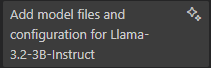
\includegraphics[width=0.5\linewidth]{figures/commit.png}
    \label{fig:enter-label}
\end{figure}
\newline
Ho accettato quanto proposto ed eseguito il Commit.
Quanto è riuscito a fare Copilot è strabiliante e allo stesso tempo un poco avvilente, in pochi istanti ha analizzato il contesto dando come output una risposta semplice ma coerente rispetto a quanto cambiato.
Lavorare in questo modo mi ricorda quando diversi anni fa, compilando La settimana enigmistica, cercavo di risolvere \textbf{senza nessun aiuto} i vari cruciverba ma avendo sempre la consapevolezza di poter guardare la soluzione se necessario.
\newline
L'intelligenza artificiale sta rivoluzionando il modo in cui il software viene sviluppato, dando la possibilità a strumenti come Copilot di esplodere tutto il loro potenziale permettono di creare la spina dorsale di un progetto lasciando al programmatore il compito di verificare e correggere solo in parte il codice perché indirizzati e condizionati da quanto proposto. 
In progetti complessi questo non riduce il ruolo del programmatore, anzi lo eleva a compiti più precisi e complessi lasciando la stesura di parti del codice semplici e ripetitive al software stesso.
Sapere cosa chiedere e formulare correttamente le domande al LLM è fondamentale, non dando nulla per scontato esplicitando nel dettaglio con parole chiave mirate come deve essere realizzato il codice.
Altro compito complesso per il programmatore è non farsi troppo ammaliare dalle soluzioni proposte perché non sempre necessarie per quanto richiesto oppure diversa da quanto già conosciuto per realizzare una determinata funzione.
Conoscere nuovi modo di operare è molto stimolante ma comporta test e tempo che a volte non è sempre disponibile.
Il programmatore deve sempre cercare di avere il giusto controllo del progetto accettando generazione del codice automatica solo dove consapevole di quanto proposto e gestibile anche in casi di revisione e manutenzione.

\paragraph{Structure of the Thesis}

\note{At the end, describe the structure of the paper}

\chapter{State of the art}

I suggest referencing stuff as follows: \cref{fig:random-image} or \Cref{fig:random-image}

\begin{figure}
    \centering
    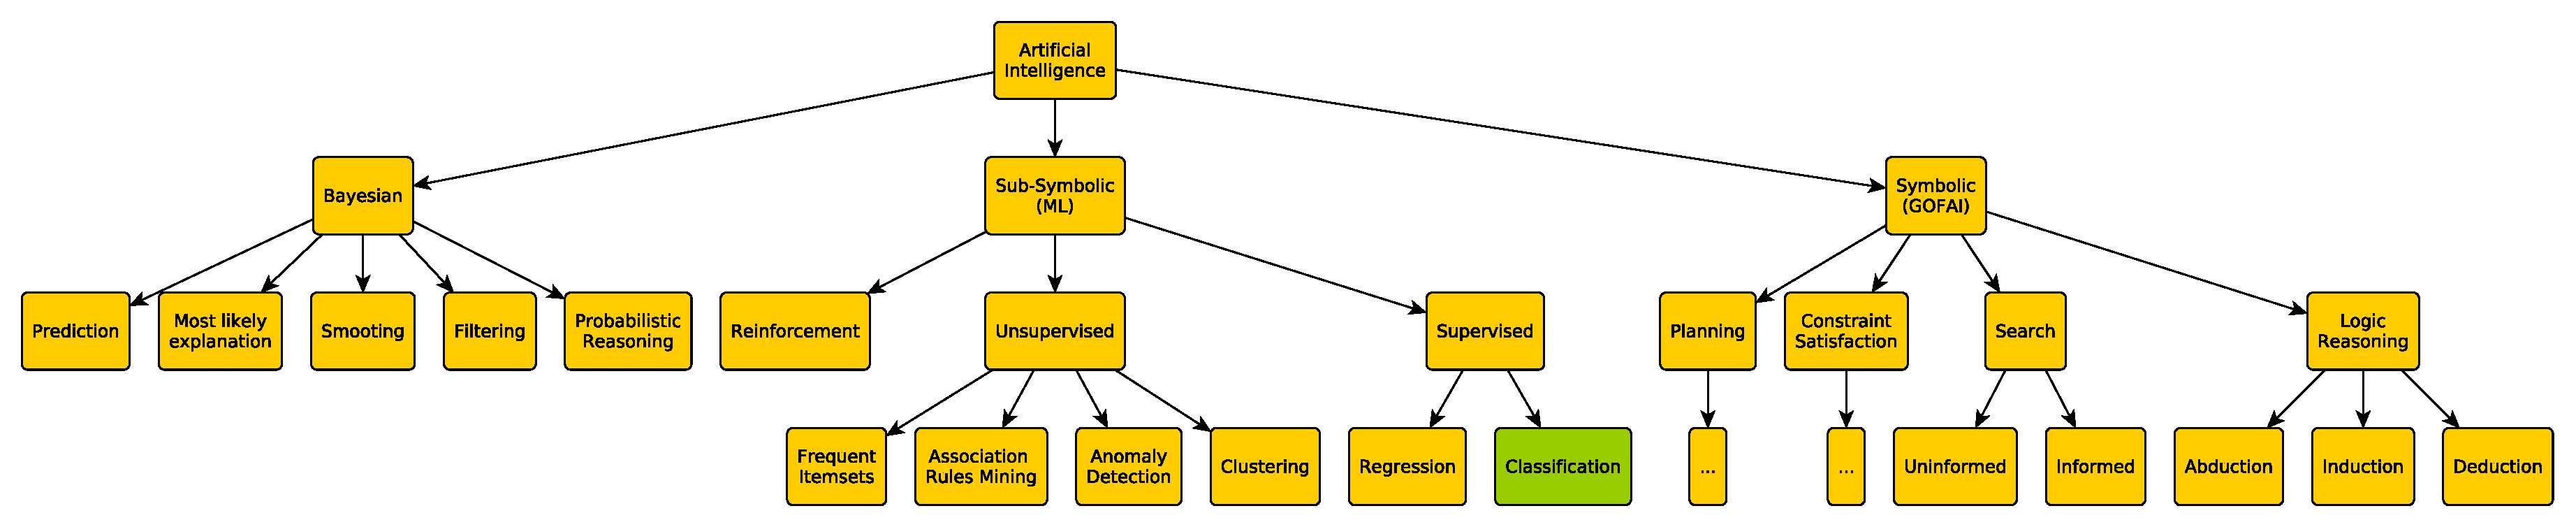
\includegraphics[width=.8\linewidth]{figures/random-image.pdf}
    \caption{Some random image}
    \label{fig:random-image}
\end{figure}

\section{Some cool topic}

\chapter{Contribution}

You may also put some code snippet (which is NOT float by default), eg: \cref{lst:random-code}.

\lstinputlisting[float,language=Java,label={lst:random-code}]{listings/HelloWorld.java}

\section{Fancy formulas here}

%----------------------------------------------------------------------------------------
% BIBLIOGRAPHY
%----------------------------------------------------------------------------------------

\backmatter

\nocite{*} % Remove this as soon as you have the first citation

\bibliographystyle{alpha}
\bibliography{bibliography}

\begin{acknowledgements} % this is optional
Optional. Max 1 page.
\end{acknowledgements}

\end{document}
